\chapter{Background} \label{chap:backAndPb} %and Problem description
\begin{bibunit}[ieeetr]
\minitoc
\vspace{2cm}
%
\noindent
\begin{minipage}[c]{0.3\textwidth}
\centering
\includegraphics[width=\textwidth]{carsharing}\\
~\\
\includegraphics[width=.7\textwidth]{cube2}
\end{minipage}
\hfill
\begin{minipage}[c]{0.76\textwidth}
\begin{abstract}
This chapter is dedicated to carsharing systems.
A description of their operational principles and a brief history are firstly presented.
More particularly, some specificities and characteristics highlight their legitimacy as interesting solutions to actual transportation issues.
Then, an overview of the related literature is given.
It addresses numerous problems from demand modelling to system management.
Specific topics about system design will be given in the next chapters.
The chapter follows with the description of a random generator produces data for one-way carsharing systems.
Assumptions, operating principles and outputs are especially detailed.
Finally, a summary and some outlooks are provided at the end of the chapter.
\end{abstract}
\end{minipage}

\newpage
\section{Carsharing systems} \label{sec:carsharingSystems}

% a mettre en intro
% $>$ Why sharing is a good solution ?
% Recent mobility surveys highlight a decline in the use of private vehicles.
% The number of daily trip by car is decreasing in urban areas.
% Vehicle sharing systems, as bike sharing or carsharing systems, are now more and more widespread and popular in dense urban cities.
\subsection{Principles and brief history}
The main idea of carsharing is to share a fleet of cars between users.
Basically, it's a model of car rental where people rent cars for short periods of time.
Carsharing systems are mainly intended for occasional drivers whom gain the benefit of private vehicle use without the costs and responsibilities of ownership \cite{shaheen_carsharing_1998}.
Its principle is based on the vehicle usage rather than vehicle possession.
Costs related to insurance, maintenance, fuel (or electricity), taxes, depreciation, etc. are supported by car owners, \ie mostly cooperative organizations or private operators.
They differ and have to be distinguished from traditional auto-rental services mainly because they are oriented to short-term rentals and fuel costs are included in the rental fee.
Mainly located in dense urban areas, they contribute to fill the gap between existing modes of transportation \cite{louvet_enquete_2013}.

\medskip
Nowadays, there are many implementations of carsharing systems adopting many different forms but generally, individuals access vehicles on an as-needed basis by joining an organisation that maintains a fleet of vehicles (essentially cars and light trucks) in a network of locations.
These are usually deploy in the vicinity of public transport stations, neighbourhoods, employment centres and universities \cite{shaheen_carsharing_1998}.

\bigskip
Although the concept of carsharing is constantly evolving, one of the most concise definition could be the one given by \cite{millard_ball_car_sharing_2005} which defines carshaing as
\begin{quote}
``a membership program intended to offer an alternative to car ownership under which persons or entities that become members are permitted to use vehicles from a fleet on an hourly basis.''
\end{quote}
More recently, in 2010, the french law defined carsharing systems under these terms :
\begin{quote}
``Carsharing is the pooling of an inland transport motor vehicles fleet for the benefit of subscribers. Each one of them can access a driverless vehicle for the ride of his choice for a limited time.'' \cite{cs_loi_2010}
\end{quote}

\bigskip
The first experiment of carsharing is identified in \cite{shaheen_short_1999} as Sefage, a Swiss company created in 1948.
For a variety of reasons, almost all effort at organising carsharing organisations resulted in failure until the early 1990's.
Different causes has been discussed to explain the origins of these common failures.
The list includes excessive financial costs, low demand, service quality deterioration, technological limitations, as well as a restricted service area and a lack of government support \cite{harms_emergence_1998, cousins_theory_2000}.

\medskip
Since then, many schemes of the system have been implemented and the basic concept of carsharing has evolved in many ways.
Over time, profit-making organisations have emerged as the most important actors in the carsharing market, even though the number of non-commercial and cooperative organisations is still the largest.
Lessons learned from unfortunate experiences combined with technological advances helped launching new carsharing programs.
Historically, first successful systems started in Europe.
Their development has highly contributed to spread and confirm the viability of vehicle-sharing systems across the world.
Today, the actual world's leader carsharing company is Zipcar.
Founded in 2000, its global vehicle fleet exceeds $12,000$ vehicles and $950,000$ members, mainly in the US \cite{zipcar_website}.

\medskip
Last decade has recorded the highest carsharing market growth.
In 2007, the total worldwide number of carsharing members was estimated to $348,000$ and the shared fleet of vehicles to nearly $11,700$ \cite{shaheen_growth_2007}.
Almost ten years later, in 2014, these numbers are approximated to $4,94$ millions ($\simeq \times 14$) and $92,200$ vehicles respectively ($\simeq \times 8$) \cite{statista_carsharingNumbers}.
Numerous programs are launched here and there among all continents.
It continues to expand in large part due to advanced technologies whose the greatest representatives are surely smart-phones.
Besides, incentive public policies allows private firms to reserve public on-street parking making the service more convenient and attractive.
Propitious indicators and worldwide experts anticipate further development for the forthcoming years \cite{shaheen_carsharing_2013}.

%%%%%%%%%%%%%%%%%%%%%%%%%
% a suivre : les types de carsharing et l'impact sur la société


% If the organisation renting the fleet may be , most of them are today run by a company managing the system. % a reformuler
% , as peer-to-peer carsharing for instance,

% (présentation CS)



\subsection{Carsharing models}
In this thesis, we focus on carsharing systems managed by private operators.
Three different models called respectively 'Round-trip', 'One-way' and 'Free-floating' can be find around the world.
They can be distinguished by their constraints related to the use of vehicles and the fact of having or not stations.
In order to access the service, carsharing companies generally required members to pay a yearly registration fees.
Sometimes it is a deposit that is refunded when membership ends.
Then, a monthly rate based on the time spent on roads and the distance travelled testifies to the personal usage of each member.

\medskip
The technology provided by the operator can vary enormously.
In Europe, most operator offer different kind of vehicles, from small city cars to large cargo vehicles.
Generally, members have access to vehicles on-the-go using smart cards or PIN (personal identification number).
They can also make a reservation online or using (smart)phones to guarantee the availability of a vehicle.
The service can sometimes be related to public transport, offering a large mobility supply to individuals.

\medskip
Round-trip and one-way systems are said \textit{station-based}.
They involve a small to medium fleet of vehicles, available at several stations, to be used by a relatively large group of members \cite{shaheen_short_1999}.
Vehicles are dispersed all across the city through many indicated stations, where a fixed number of parking places stores the vehicles.
Generally, carsharing companies dispose of their own dedicated parking lots situated on-street or off-street according to contractual arrangement with the entity (private or public) managing the parking.
The number of lots can varies according to the size of the system and the available urban space, but since carsharing is mainly implanted in dense urban areas, stations are often small.
In Paris, for instance, the number of parking places is between $4$ and $7$ \cite{autolib_rapport_2014}.
Also, station-based systems can provide additional specific infrastructure if necessary.
The carsharing service Autolib' in Paris, offers charging points for electric vehicles and kiosks for customer service.


\subsubsection{The Round-Trip system}
\begin{wrapfigure}[6]{r}{3cm}
\vspace{-.4cm}
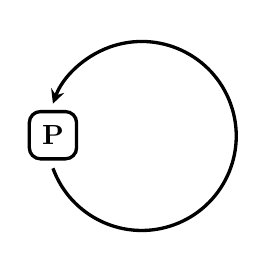
\begin{tikzpicture}[scale = .6]
\draw[very thick, rounded corners] (-.5,-.5) rectangle(.5,.5);
\draw node at (0,0){\textbf{P}};
%\fill[black] (0,0) circle (.5);
\draw[very thick, ->, > = stealth,] (0,-.7) arc (-160:160:2);
\end{tikzpicture}
\end{wrapfigure}
Historically, the first carsharing scheme to be implemented was the round-trip system.
As such, it is today the best established commercially and has been largely studied.
Basically, It requires users to return vehicles to the station they were picked up.
Such systems are simple to design since the incoming demand in each station is sufficient to plan vehicle stocks.
The user behaviour is mainly oriented to leisure and household shopping purpose \cite{barth_shared_use_2002, costain_synopsis_2012}.


\subsubsection{The One-way system}

\begin{wrapfigure}[6]{l}{3cm}
\vspace{-.4cm}
\centering
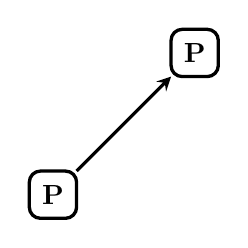
\begin{tikzpicture}[scale = .6]
\draw[very thick, rounded corners] (-.5,-.5) rectangle(.5,.5);
\draw node at (0,0){\textbf{P}};
\draw[very thick, rounded corners] (2.5,2.5) rectangle(3.5,3.5);
\draw node at (3,3){\textbf{P}};
%\fill[black] (0,0) circle (.5);
%\fill[black] (3,3) circle (.5);
\draw (.5,.5) edge[very thick, ->, > = stealth,] (2.5,2.5);
\end{tikzpicture}
\end{wrapfigure}

One-way carsharing scheme is more flexible than round-trip.
It allows users to pick up a vehicle from a station and return it in a different one, possibly distinct from the origin.
Unfortunately, this greater flexibility comes with hard operational problems due to the uneven nature of the trip pattern in urban areas.
Indeed, empty stations exclude potential requests to be satisfied.
Conversely, crowded stations do not allow an incoming vehicle to park.
Thus, the system imbalance must be corrected so that vehicles can be relocated to suitable places.
This problem referred as the vehicle imbalance problem is discussed thereafter.
%, listed and described below,

However, let notice that despite these difficulties for the operator, one-way system captures more trips than the alternative system thanks to this flexibility which is a critical factor to join a carsharing scheme \cite{efthymiou_which_2012}.


\subsubsection{The Free-floating system}

\begin{wrapfigure}[6]{r}{3cm}
\vspace{-.4cm}
\centering

\begin{tikzpicture}[scale = .6, > = stealth,]
\fill[black] (0,0) circle (.5);
\foreach \angle in {0,45,...,315} {
\draw (\angle:0.6) edge[very thick, ->, > = stealth,] (\angle:2);
};
\end{tikzpicture}
\end{wrapfigure}

Nowadays, many carsharing schemes have been tested and experimented.
Although first ones have been station-based designed, we have witnessed in the last decade the emergence of carsharing models without stations.
The user can picked up on-street parked vehicles owned by the system operator and parked on any legal parking space within a defined area.
This new feature comes with the propensity to assign more and more flexibility to the service.
Point-to-point free-floating carsharing (often referred to as flexible carsharing) corresponds to a sharing scheme where usage is typically spontaneous.
Vehicle reservations are mostly made several minutes in advance.
The system operator ensures a service quality based on vehicle maintenance and available parking places.
The largest free-floating system is operate by car2go mainly in Germany.
In 2015, the service account for more than one million members.
% whereas the third one, appeared recently, offers more flexibility 

\subsection{Positive impacts}
% on the transportation system
As an innovative alternative to private car ownership, carsharing is a interesting trade off between distance and flexibility.
On the one hand, the car provides the freedom to cover entire urban areas.
Even with electric vehicles, for which the autonomy is limited, distances of more than $150$ kilometres can be considered.
On the other hand, the fact that cars are available on-demand relieves users from the rigidity of public transport timetables.
Moreover, station-based carsharing systems aim at reducing the time spent at searching for a parking lot, which is often important in dense urban areas.
In France, its contribution to the global congestion is evaluated between $5$ and $10$\%  \cite{stationnement_intelligent_cerema}.
As a consequence, carsharing is now considered as an attractive transportation mode filling the gap between traditional public transport and private vehicle use.

\medskip
In the last decade, several authors have showed that carsharing systems have positive impacts on users, the transportation system and the environment.
Although not all of these commonly attested benefits are documented with empirical data, next sections present substantial agreements about carsharing on the urban mobility, financial gains and the environment.


\subsubsection{Urban mobility}

The carsharing economic model is founded on the use of the vehicles.
The cost for moving from point A to point B depends on the distance and the time the user spend on the road.
As such, carsharing infers on user behaviours, whom aligned their car usage on those criterion, and therefore provides greater incentive for members to be selective about driving.
In other words, members have a heightened awareness of travel costs and tend to reduce unnecessary trips to save money.
% nb km decrease
A study conducted in 2004 reports that carsharing users reduce their vehicle kilometres traveled (VKT) -- or vehicle miles traveled (VMT) -- by $50$\% after joining the organisation \cite{cervero_city_2004}.
More recent result evaluated this decrease to $27$\% in 2011 \cite{martin_greenhouse_2011}.
% car ownership decreases
Another often observed outcome of carsharing is a fall in car ownership rates.
The number of vehicles per household is a half lower for carsharing users than private cars users \cite{martin_impact_2010, ter_schure_cumulative_2012}.
When carsharing responds to mobility needs, members postpone or even drop the idea of buying a new car \cite{martin_impact_2010, sioui_carsharing_2013}.

\medskip
% vehicle utilization rate increases
Globally, each shared vehicle is used more efficiently \cite{litman_evaluating_2000, schuster_assessing_2005}.
Because of higher utilization rates than single-user private vehicles, they spend more time on the road and less time parked (which represent for a private car almost 95\% of its total use time, as mentioned in \cite{transflash_2013}).
A direct consequence in the medium to long-run is that parking requirements in dense areas should also decrease \cite{mitchell_reinventing_2010}, freeing urban space.
% nb of vehicles decreases 
Those observations argue that carsharing decreases the number of vehicles on the road.
However, the less vehicles on the road, the better the traffic fluidity is.
Thus, carsharing also helps reducing traffic congestion at peak times.


\subsubsection{Economical aspects}
General costs related to car ownership are commonly split into fixed and variable expenses.
According to the total distance travelled, driving habits or local parking costs, the variable costs might be very different from one car owner to the other.
However, the share of fixed costs, such as the purchase price of the vehicle, its depreciation over time or insurance, still remains predominant \cite{cout_reel_auto}.
In this context, embracing a carhsharing service where the price only depends on the vehicle usage can grants its users the car mobility at interesting costs.

\medskip
Nevertheless, those benefits are not relevant for every car user.
Basically, the less the car is used, the more carsharing services become interesting.
With respect to local costs, researches have shown that car users driving less than $10,000$ kilometres per year (as much as \hbox{$15,000$ km/y}) could save money using carsharing \cite{litman_evaluating_2000, prettenthaler_ownership_1999}.

% using carsharing is considered as a complementary affordable mobility solution that may replace the car ownership for some individuals.


\subsubsection{Environmental effects}

Obviously, reducing the number of cars on the road have have positive environmental effects.
Results of recent survey studies seem to indicate that greenhouse gas (GHG) emissions are largely reduced 
\cite{martin_greenhouse_2011, firnkorn_what_2011}.
These results are reinforced with the recent emergence of electric vehicles, for which CO2 emissions are largely reduced.
Besides, they provide noise reduction since electric cars are quitter than thermal ones.
Moreover, the reduction of parking demand can be used to reallocate the land for additional green spaces, new mixed-use development, or other community needs \cite{cohen_carsharing_2008}.


\subsection{Related problems}

Academic literature on carsharing systems is very prolific since a couple of decades.
Inspired and motivated by their recent diffusion, researchers report on a large variety of topics covering system design, system management, social characterization, logistic, etc.
Approaches use both qualitative and quantitative methodologies.
Addressed problems are generally segmented into the following categories \cite{ciari_sharing_2012}:
\begin{itemize}
\item Market analysis,
\item Impacts of carsharing,
\item Carsharing operations and management.
\end{itemize}

Although slightly outdated, this categorization is inspired by a literature review of Millard-Ball et al. \cite{millard_ball_car_sharing_2005}.
A complete updated overview on problems arising in such systems can however be found in the work of Jorge et al. \cite{jorge_carsharing_2013}.

\medskip
In a previous talk, we have already given an overview of the positive impacts carsharing can provide.
In addition, this thesis is dedicated to optimal system design and focus more particularly at the optimal dimensioning and station locations.
In the next chapters, we give a deeper look about current results on those particular topics.
The following sections will consequently focus on market analysis and problems related to system operations and management.


\subsubsection{Social aspects and demand modelling}
Who are the users and why they use the service are probably the major addressed questions about carsharing.
Most works aim at characterize and analyse members' behaviour, so that the specific transportation demand associated to carsharing can be estimated mathematically.
In the domain of transportation, this popular topic is known as the \emph{demand modelling}.
The outputs of such models are then used to deal with operational research problems and system management.
By doing so, carsharing decision makers are endowed with accurate inputs helping the resolution of other problems more efficiently.

\medskip
Unfortunately, the ability to predict the demand for carsharing still is a quite challenging and hard topic.
Several reasons, manly related to the uneven nature of the demand, can explain why economists and modellers struggle to propose accurate tools \cite{danielis_potential_2015}.
First, the carsharing demand is highly dependant on the mobility patterns, which is partly recurrent (such as home/work travels or study commuting) and partly random.
Secondly, involved decisions leading to carsharing joining are many and various.
In addition, they include both quantitative and qualitative criterion.
They not only depends on the price, the quality, the travel time, the trip distance and comfort, but also on the supply of the other competing or complementary modes.
Finally, some side effects due to the dynamics of the system itself may influence the demand.
The evolution of the service quality over time (\eg the availability of vehicles or parking places) can fluctuate the incoming demand, making its prediction even more complex.

\medskip
Using statistical data and user surveys, most studies have nevertheless demonstrated important tendencies.
Basically, the average carsharing member has the following characteristics
\cite{brook_carsharingstart_2004}
\cite{millard_ball_car_sharing_2005}
\cite{lane_phillycarshare_2005}
\cite{zheng_carsharing_2009}
\cite{costain_synopsis_2012}
\cite{efthymiou_which_2012}:
\begin{itemize}
\item age between mid-30s to mid-40s,
\item people highly educated and environmentally aware,
\item income higher than average.
\end{itemize}

\bigskip
Regarding the geographical aspects of carsharing, its usage is highly correlated with the use of public transports and most successful applications are running in dense urban areas \cite{cervero_city_2003, millard_ball_car_sharing_2005, burkhardt_who_2006}.
Moreover, the accessibility to the stations, in terms of distance between home/work and the nearest station, is identified as a critical factor to joining a carsharing system \cite{zheng_carsharing_2009, costain_synopsis_2012, efthymiou_which_2012}.


\medskip
Identify the main factors which generate and influence the demand greatly contribute to give a good prediction of a carsharing service.
Stillwater et al. \cite{stillwater_carsharing_2009} compared the use of carsharing vehicles to build-environment and demographic factors in the US.
They concluded that the most significant variables were: the street width ($-$), the provision of a railway service ($-$), the percentage of drive-alone commuters ($-$), 
the percentage of households with one vehicle ($+$), and the average age of the stations ($+$).
Signs ($-$) or ($+$) are used to indicate whether the indicator is negatively or positively related to the carsharing demand.
The street width and the percentage of drive-alone commuters may not have a clear intuitive explanation at first sight although those metrics are significantly related to the level of carsharing demand.
The authors postulated that street width contains informations about pedestrian environment (where narrow streets are more pedestrian friendly) and about the land use in general (narrow streets trend to denote older residential or mixed-use development) which make sense since carsharing and walking behaviour are known to be strongly related \cite{cervero_city_2003}.
The proportion of drive-alone commuters are negatively related because these people are in general already vehicle-owners.
Indeed, a high level of commuting vehicles tend to signify that the neighbourhood has a poor public transit or is already provided with high-density mode amenities.


\medskip
Another study conducted by Ciari et al. \cite{ciari_estimation_2013} uses an activity-based micro-simulation model to estimate travel demand.
The authors also try to understand the effects of a carsharing system on urban mobility, considering others transportation modes such as public transport, car, bicycle and walking.
They suggested and evaluated a carsharing demand model using an open-source activity-based multi-agent simulator called MATSim \cite{matsim_webPage}.
The framework simulates the daily life of individuals (agents) and produces travel demand as a side product.
The system process iteratively computes transportation plans and traffic flow simulations until a relaxed state is reach.
A transportation plan is a list of transportation modes deduced from a user activity-chain.
Activities planned during the day by a user are selected with respect to its socio-demographic attributes.
An aggregated cost function (including carsharing as a transportation mode in itself) returns a score, evaluating quantitatively the plans of each user.
The agents continuously try to improve their score varying their departure time, transport modes, routes and location of some activities.

The authors led to a modal split model giving plausible results in comparison with real \mbox{data -- the} urban area of Zurich, Switzerland.
According to the access to the cars and the time dependent fee structure, the model captures the proportion of the total transportation demand that could use carsharing.
Although they observed general pattern of mobility at macro-scale, the authors also pointed out that results are context specific and computationally intensive.


\bigskip
Actually, in most cases, studies are context specific.
Trip patterns and travel behaviour can be different from one country to another since it is related to local and regional characteristics (culture, habits, etc.), making the standardization more complex.
Furthermore, carsharing demand estimation has not so far been addressed in the literature for one-way carsharing systems, and a relevant model for such models is nowadays not available \cite{jorge_carsharing_2013}.
This is a real challenge for the future since it's reasonable to think that one-way carsharing systems will be increasingly present in the coming years.

%\cite{leclerc_unraveling_2013} (comportement des utilisateurs carsharing)\\


\subsubsection{The vehicle imbalance problem}
In one-way systems, one of the most challenging problem deals with \emph{vehicle relocations} strategies.
Unlike round-trip models, the departure station and the arrival station are not necessary identical.
As a result, the dynamics of the system may conduct to critical situations.
On the one side, empty stations prevent the members to find a vehicle, whereas on the other side, full stations prevent them to park.
This property induces imbalance issues to the system and a lot of efforts are made to understand the dynamics involved and find possible solutions to handle it.

\medskip
A first intuitive approach for solving the vehicle imbalance problem is to consider that the operator have to do periodic vehicle relocation operations among stations.
In general, carsharing operator recruit employees (also referred as \emph{jockeys}) to balance the system and avoid critical situations.
Some studies, using discrete event simulation models, help operators to manage their systems minimizing the available resources (such as vehicles and staff members), while maintaining certain levels of service \cite{barth_simulation_1999, kek_relocation_2006, kek_decision_2009}.
More specifically, the model presented in \cite{kek_decision_2009} has been tested and validated using real data, a one-way carsharing company in Singapore called Honda ICVS.
Proposed solutions aimed at reduce the staff cost of about $50$\%.

\medskip
Other authors have explored the problem under the optimization methods perspective.
For instance, the model proposed in \cite{nair_fleet_2011} is a stochastic mixed-integer programming (MIP) model with the objective of generating least-cost vehicle redistribution where the demand is known probabilistically.
In \cite{smith_rebalancing_2013}, the authors find the optimal rebalancing strategy solving two different linear programs in a fluid model of the system: one in order to minimize the number of rebalancing vehicles, the other for minimizing the number of rebalancing drivers (jockeys), considering that the number of waiting customers remains bounded.
The authors stated that the ``two objectives were aligned'' and concluded that, for Euclidean network topologies, the numbers of jockeys the systems required is between 1/4 and 1/3 of the total number of vehicles.

\medskip
Very recently, \cite{zakaria_optimization_2015} focuses on the logistic aspects of relocation operations, including the number of jockeys, and specific day-times for relocation and shifting operations.
Different relocation policies are especially studied.
The better performance at minimizing the number of rejected demands was obtain using a relocation policy where jockeys can have information on the future state of the system.
Those anticipations were calculated using historical data of the system and predictions. % Better results where m
The author suggest that applying policies based on intuitive decisions, such as distance to stations and number of cars at stations, without taking into consideration the effect of these relocation operations on the whole system will not be very efficient in reducing the number of rejected demands.

\medskip
Another innovative approach is to consider that clients can be used to relocate the vehicles through various incentive mechanisms, mainly based on rewards.
Prices could be used in order to encourage users to sign up to ``trip splitting'' and ``trip joining'', as showed in \cite{barth_user_based_2004}.
The principle is very simple: when users want to travel from a station with shortage of vehicles to another one with an excess they are prompted to share the ride in a single vehicle (trip joining), while, conversely, when they wanted to travel from a station with too many vehicles to one with a shortage they are encouraged to drive separate vehicles (trip splitting).
Despite the fact that this strategy effectively balances the system in theory, it relies on assumptions that may be unrealistic in practice.
For instance, it's not relevant if a majority of travellers value privacy and convenience over minor cost saving.
Also, this scheme does not work if trip-joining policies make carsharing similar to carpooling, which has severe sociological barriers associated with riding with strangers, mainly for safety and security reasons \cite{chan_ridesharing_2012, correia_carpooling_2011}).
Finally, with respect to trip splitting, impossibilities could occur if users simply do not want to be divided.


\section{A generator addressing the lack of data} \label{csgeneratorDescription}

As pointed out earlier, the carsharing demand is hard to model and forecast.
As far as we know, there is no available model for one-way carsharing in the literature which is not context specific.
Besides, operational data from carsharing operators are not accessible.
Although some global indicators of the service are sometimes reported (such as the stations' locations, the number of vehicles or the number of daily requests) no private company release the details of the registered demand, mainly for users' confidentiality reasons.

\medskip
The problems addressed in this thesis deal with the design of a one-way carsharing system.
In this work, we consider the carsharing demand as an input of the addressed problems and, as such, need to be evaluated.
This section presents the mechanics of a random data generator developed during the thesis.
Basically, the generator produces time-dependant one-way carsharing demand among a set on randomly positioned stations.
The provided data are used to evaluate the developed models proposed in the next chapters.
The generator can be downloaded freely as an open-source software at \cite{csgen}.
Figure \ref{fig:csgen-mainFrame} illustrates the main frame of the software.
We hope that it could help the research community, stimulate system design implementations and provide benchmark data to compare methodologies.

%\subsection{Demand modelling}
%\cite{modele_deplacement_dreif_2008}\\

\subsection{Assumptions}

\begin{figure}[!h]
\centering
\includegraphics[width = .75\textwidth]{csgen-mainFrame}
\caption{Main frame of the generator.}
\label{fig:csgen-mainFrame}
\end{figure}

% Discrete time
Some data produced by the generator are time-dependant.
The purpose of the generator is to provide temporal data during an average day.
Carsharing demands and travel times are then defined over a $24$ hours period, segmented into $\nbTimeSteps \in \N$ discrete time-steps.
The total number of time-steps is user-settable.
It can vary from $24$ to $1440$, representing respectively a time-step period of one hour and one minute.

% Constant vehicle speed
\medskip
The vehicle speed is assumed constant during a trip.
Although congestion is not directly considered in the model, travel times are penalize during rush hours.
Two weight factors (one for the morning, one for the evening) allow to extend any trip duration if it is performed during defined time windows.

% Operation chain
\medskip
Finally, it is also assumed that the generator neglects the time needed for some operations.
For instance, the time needed to park a vehicle, borrow it or plug it into a charging point in the case of electric vehicles are not considered.


\subsection{Station positioning}
The first phase positions $\nbStations \in \N$ carsharing stations within a given territory.
The area is modelled as a square, only defined by its side length expressed in metres.
Then, two distinct methods, called respectively the \emph{uniform} method and the \emph{centroid} method, spread the stations among the territory.
The uniform method merely positions randomly the stations, assigning uniform random values to the station's coordinates.
The centroid method positions stations over two distinct zones: a central area (in general representing the center of the city) included in a larger one (representing the suburbs area), both defined as a square.
The generation algorithm takes two additional parameters: the percentage of total area the center must represent and the probability that a station is contained in the center.
Once the geographic division is made, every station is then positioned randomly in the area where it belongs. 
Finally, the maximum size for each station is randomly generated using a discrete uniform distribution over an integer interval given by the user. %$[Z_{\min}, Z_{\max}]$


\subsection{Demand generation}
The second phase generates randomly $\nbDemands \in \N$ demands over time between stations.
In a first step, the generator schedules and distributes randomly each request over time.
The random demand distribution can be specified through a dedicated frame where the user can tune every level demand on an hourly basis.
Because levels are considered relative to each other, their exact value are not relevant.
The random distribution is obtained normalizing all the values. % \ie ${\cal P}(t) = Dem(t) \slash \sum_{t}{Dem(t)}$.
In practice, most profile distributions are very similar to the one presented in Figure \ref{fig:plotDemandProfile} where two noticeable picks during morning and evening demarcate the symmetrical mobility pattern in dense area.

\medskip
In a second step, the generator identifies origins and destinations of each temporal demands.
Usually, in urban context, the demand goes globally in the same direction: from the suburbs to the center during the morning and from the center to the suburbs the evening.
Both morning and evening rush hour slots (traffic peaks) are settable.
As depicted in Figure \ref{fig:plotDemandProfile}, the morning rush is usually between $7$ and $9$ o'clock whereas the evening rush is between $15$ and $19$ o'clock.
A fixed demand proportion during rushes can be specified by the user.
The generator finally calculate the origin and destination stations with respect to the departure time of each demand.
The travel time is deducted from the distance between stations and the average car speed.
As stated previously, the time is penalized in case of traffic peaks.


\begin{figure}[t]
\centering
\begin{tikzpicture}[>=stealth, thick, scale = 1]
%
\begin{axis}[ % DEMAND PROFILE
	height = 10cm,
	width = 15cm,
	axis x line = bottom,
	axis y line = none,
	xlabel = {Hours of the day},
	xtick={0,2,...,24},
	xticklabels = {0h, 2h, 4h, 6h, 8h, 10h, 12h, 14h, 16h, 18h, 20h, 22h, 0h},
	xmin = -0.5,
	xmax = 24.5,
	ymin = 0,
	ymax = 95,
	legend entries = {~Demand profile},
	legend style = {at = {(0,1)}, anchor = north west, },
	legend cell align = left,
]
\fill[red!20, ] (axis cs:7,0) rectangle (axis cs:9,100);
\fill[red!20, ] (axis cs:15,0) rectangle (axis cs:19,100);

\draw (axis cs:7,5) edge[red, <->, line width = .7pt] (axis cs:9,5);
\draw (axis cs:15,5) edge[red, <->, line width = .7pt] (axis cs:19,5);
\draw node[rotate = 90, red, anchor = west] at (axis cs:8,7){Morning Rush};
\draw node[rotate = 90, red, anchor = west] at (axis cs:17,7){Evening Rush};

\addplot[mark = none, draw = blue!60, smooth, line width=2pt] table [col sep=semicolon, x=TS, y=DEMAND]{tikz/DemandProfile.csv};
\end{axis}
\end{tikzpicture}
\caption{Demand profile over the day.}
\label{fig:plotDemandProfile}
\end{figure}


\subsection{Outputs}

The data produced by the generator are saved as XML files.
Two markup sets hold all the required information.
The first one, dedicated to stations, reports the following data:
\begin{itemize}
\item id: the station ID,
\item xPos, yPos: the station geographical coordinates,
\item maxSize: the maximum number of available parking lots in the station.
\end{itemize}
The second set, dedicated to demands, includes the following data: 
\begin{itemize}
\item id: the demand ID,
\item idsOrigin, idsDestination: The IDs of departure and arrival stations,
\item nbDemand: the number of individuals requested a vehicle,
\item departureTime, arrivalTime (expressed in number of time-steps): time of the request and time of the expected arrival at destination.
\end{itemize}

Figure \ref{fig:csgen-output} gives an example of an instance generated for $50$ stations and $500$ demands over the day.


\begin{figure}[!h]
\centering
\includegraphics[width = \textwidth]{csgen-output}
\caption{Generator output.}
\label{fig:csgen-output}
\end{figure}



%Figure \ref{fig_randomStationPositioning} illustrates the positioning of $100$ stations in the Paris area where $p_{center}$ is set to $10\%$ and $p_{concentration}$ to $35\%$.

%\begin{figure}[h]
%\centering
%\includegraphics[scale=0.25]{stationGenerationExample}
%\caption{Random station positioning over the city of Paris and its region}
%\label{fig_randomStationPositioning}
%\end{figure}


\section{Synthesis and outlooks}

In this literature overview, we have seen that carsharing systems can be a real alternative to private vehicles.
Mainly located today in dense urban area, they provide positive impacts not only on the environment but also on urban mobility.
A rich literature on these topics tend to demonstrate that congestion, pollution and parking demand can be greatly enhanced with such systems.
Providing an interesting trade off between the covered distance and flexibility, carsharing systems are now recognized as good solutions to deal with urban transportation problems.

\medskip
Three carsharing schemes, called respectively round-trip, one-way and free-floating, are popular worldwide.
Constraints on trips as well as the provided system infrastructure (stations) distinguish one from the other.
The current trend is to offer more flexibility by allowing one-way trips without the obligation to parked at fixed places.
In this thesis, we focus on one-way carsharing systems managed by private operators.
Those station-based services allow the user to picked up a vehicle at any station and return it in a different one.


\medskip
The recent emergence and diffusion of carsharing have raised various research topics covering, among other, demand forecasting, network design and system management.
A first sight at the demand characterization show that the typical carsharing user is relatively young, well educated and has an income higher than average.
Actually, studies trying to figure out who the users are greatly help to design accurate demand forecast models.
This social characterization is essential and directly related to demand modelling research.
The addressed approaches vary from linear regression and cluster analysis to more sophisticated method such as activity-based microsimulation.
Unfortunately, articles reviewed on demand estimation have generally not taken into account the one-way option.
Moreover, attempts to estimate the proportion of travellers that could join and use a carsharing service are very often context specific which limits the scope and the applicability of the results.
Since one-way systems will continue to spread out in the near future, it will be crucial to develop realistic models that can handle those specific mechanics in a multimodal environment.


\medskip
We have presented in the end of this chapter a random demand generator for one-way carsharing systems.
The development of the generator was originally motivated by the lack of available data.
The resulting outputs produced by the tool emulate a potential carsharing systems with stations and temporal demands during a representative period of $24$ hours.
The source code is freely accessible \cite{csgen} and we aspire that it could help and stimulates further research.


\medskip
Regarding the system management aspects, the main problem faces carsharing operators is how to determine and maintain the right number of vehicles in stations so that the system efficiently satisfies the requested demands.
This problem, referred as the vehicle imbalance problem, involves vehicle repositioning strategies performed by employees of the operator (jockeys) in order to provide the best operational configuration.
Simulation and mathematical programming are the two most commonly used techniques for dealing with this problem.
Many studies stated that the ability to balance vehicles between stations is crucial for the overall system performance.
Indeed, good relocation strategies allow the system operates at a reliability level that could not be achieve otherwise.


\medskip
Problems addressed in this thesis deal with the system design of a one-way carsharing system.
More precisely, how to conceive the most efficient system according to a demand estimation?
How many stations?
Where?
With how many parking slots and vehicles?
Although system design problems are addressed before system management, some inner mechanics such as vehicle relocation are still relevant to be considered.
In this chapter, we have intentionally eluded those particular topics because a specific literature review is provided in next of the thesis.

%Let's notice and emphasize that accurate outputs of the demand estimation is a paramount data for both problems.
%Actually, this last problem represents the core of this thesis and the scope of our research.
%Therefore, the next chapter will introduce more precisely the reasons why we were especially interested by those aspects and give a mathematical formulation of the problem we are working on.


\newpage
\addcontentsline{toc}{section}{Bibliography of chapter \thechapter}
\renewcommand{\bibname}{Bibliography of chapter \thechapter}
\putbib[bib/biblio]
\end{bibunit}
